\ifx\allfiles\undefined
\documentclass[12pt, a4paper, oneside, UTF8]{ctexbook}
\def\path{../config}
\usepackage{amsmath}
\usepackage{amsthm}
\usepackage{amssymb}
\usepackage{array}
\usepackage{xcolor}
\usepackage{graphicx}
\usepackage{mathrsfs}
\usepackage{enumitem}
\usepackage{geometry}
\usepackage[colorlinks, linkcolor=black]{hyperref}
\usepackage{stackengine}
\usepackage{yhmath}
\usepackage{extarrows}
\usepackage{tikz}
\usepackage{pgfplots}
\usepackage{asymptote}
\usepackage{float}
\usepackage{fontspec} % 使用字体

\setmainfont{Times New Roman}
\setCJKmainfont{LXGWWenKai-Light}[
    SlantedFont=*
]

\everymath{\displaystyle}

\usepgfplotslibrary{polar}
\usepackage{subcaption}
\usetikzlibrary{decorations.pathreplacing, positioning}

\usepgfplotslibrary{fillbetween}
\pgfplotsset{compat=1.18}
% \usepackage{unicode-math}
\usepackage{esint}
\usepackage[most]{tcolorbox}

\usepackage{fancyhdr}
\usepackage[dvipsnames, svgnames]{xcolor}
\usepackage{listings}

\definecolor{mygreen}{rgb}{0,0.6,0}
\definecolor{mygray}{rgb}{0.5,0.5,0.5}
\definecolor{mymauve}{rgb}{0.58,0,0.82}
\definecolor{NavyBlue}{RGB}{0,0,128}
\definecolor{Rhodamine}{RGB}{255,0,255}
\definecolor{PineGreen}{RGB}{0,128,0}

\graphicspath{ {figures/},{../figures/}, {config/}, {../config/} }

\linespread{1.6}

\geometry{
    top=25.4mm, 
    bottom=25.4mm, 
    left=20mm, 
    right=20mm, 
    headheight=2.17cm, 
    headsep=4mm, 
    footskip=12mm
}

\setenumerate[1]{itemsep=5pt,partopsep=0pt,parsep=\parskip,topsep=5pt}
\setitemize[1]{itemsep=5pt,partopsep=0pt,parsep=\parskip,topsep=5pt}
\setdescription{itemsep=5pt,partopsep=0pt,parsep=\parskip,topsep=5pt}

\lstset{
    language=Mathematica,
    basicstyle=\tt,
    breaklines=true,
    keywordstyle=\bfseries\color{NavyBlue}, 
    emphstyle=\bfseries\color{Rhodamine},
    commentstyle=\itshape\color{black!50!white}, 
    stringstyle=\bfseries\color{PineGreen!90!black},
    columns=flexible,
    numbers=left,
    numberstyle=\footnotesize,
    frame=tb,
    breakatwhitespace=false,
} 

\lstset{
    language=TeX, % 设置语言为 TeX
    basicstyle=\ttfamily, % 使用等宽字体
    breaklines=true, % 自动换行
    keywordstyle=\bfseries\color{NavyBlue}, % 关键字样式
    emphstyle=\bfseries\color{Rhodamine}, % 强调样式
    commentstyle=\itshape\color{black!50!white}, % 注释样式
    stringstyle=\bfseries\color{PineGreen!90!black}, % 字符串样式
    columns=flexible, % 列的灵活性
    numbers=left, % 行号在左侧
    numberstyle=\footnotesize, % 行号字体大小
    frame=tb, % 顶部和底部边框
    breakatwhitespace=false % 不在空白处断行
}

% \begin{lstlisting}[language=TeX] ... \end{lstlisting}

% 定理环境设置
\usepackage[strict]{changepage} 
\usepackage{framed}

\definecolor{greenshade}{rgb}{0.90,1,0.92}
\definecolor{redshade}{rgb}{1.00,0.88,0.88}
\definecolor{brownshade}{rgb}{0.99,0.95,0.9}
\definecolor{lilacshade}{rgb}{0.95,0.93,0.98}
\definecolor{orangeshade}{rgb}{1.00,0.88,0.82}
\definecolor{lightblueshade}{rgb}{0.8,0.92,1}
\definecolor{purple}{rgb}{0.81,0.85,1}

\theoremstyle{definition}
\newtheorem{myDefn}{\indent Definition}[section]
\newtheorem{myLemma}{\indent Lemma}[section]
\newtheorem{myThm}[myLemma]{\indent Theorem}
\newtheorem{myCorollary}[myLemma]{\indent Corollary}
\newtheorem{myCriterion}[myLemma]{\indent Criterion}
\newtheorem*{myRemark}{\indent Remark}
\newtheorem{myProposition}{\indent Proposition}[section]

\newenvironment{formal}[2][]{%
	\def\FrameCommand{%
		\hspace{1pt}%
		{\color{#1}\vrule width 2pt}%
		{\color{#2}\vrule width 4pt}%
		\colorbox{#2}%
	}%
	\MakeFramed{\advance\hsize-\width\FrameRestore}%
	\noindent\hspace{-4.55pt}%
	\begin{adjustwidth}{}{7pt}\vspace{2pt}\vspace{2pt}}{%
		\vspace{2pt}\end{adjustwidth}\endMakeFramed%
}

\newenvironment{definition}{\vspace{-\baselineskip * 2 / 3}%
	\begin{formal}[Green]{greenshade}\vspace{-\baselineskip * 4 / 5}\begin{myDefn}}
	{\end{myDefn}\end{formal}\vspace{-\baselineskip * 2 / 3}}

\newenvironment{theorem}{\vspace{-\baselineskip * 2 / 3}%
	\begin{formal}[LightSkyBlue]{lightblueshade}\vspace{-\baselineskip * 4 / 5}\begin{myThm}}%
	{\end{myThm}\end{formal}\vspace{-\baselineskip * 2 / 3}}

\newenvironment{lemma}{\vspace{-\baselineskip * 2 / 3}%
	\begin{formal}[Plum]{lilacshade}\vspace{-\baselineskip * 4 / 5}\begin{myLemma}}%
	{\end{myLemma}\end{formal}\vspace{-\baselineskip * 2 / 3}}

\newenvironment{corollary}{\vspace{-\baselineskip * 2 / 3}%
	\begin{formal}[BurlyWood]{brownshade}\vspace{-\baselineskip * 4 / 5}\begin{myCorollary}}%
	{\end{myCorollary}\end{formal}\vspace{-\baselineskip * 2 / 3}}

\newenvironment{criterion}{\vspace{-\baselineskip * 2 / 3}%
	\begin{formal}[DarkOrange]{orangeshade}\vspace{-\baselineskip * 4 / 5}\begin{myCriterion}}%
	{\end{myCriterion}\end{formal}\vspace{-\baselineskip * 2 / 3}}
	

\newenvironment{remark}{\vspace{-\baselineskip * 2 / 3}%
	\begin{formal}[LightCoral]{redshade}\vspace{-\baselineskip * 4 / 5}\begin{myRemark}}%
	{\end{myRemark}\end{formal}\vspace{-\baselineskip * 2 / 3}}

\newenvironment{proposition}{\vspace{-\baselineskip * 2 / 3}%
	\begin{formal}[RoyalPurple]{purple}\vspace{-\baselineskip * 4 / 5}\begin{myProposition}}%
	{\end{myProposition}\end{formal}\vspace{-\baselineskip * 2 / 3}}


\newtheorem{example}{\indent \color{SeaGreen}{Example}}[section]
\renewcommand{\proofname}{\indent\textbf{\textcolor{TealBlue}{Proof}}}
\NewEnviron{solution}{%
	\begin{proof}[\indent\textbf{\textcolor{TealBlue}{Solution}}]%
		\color{blue}% 设置内容为蓝色
		\BODY% 插入环境内容
		\color{black}% 恢复默认颜色(可选,避免影响后续文字)
	\end{proof}%
}

% 自定义命令的文件

\def\d{\mathrm{d}}
\def\R{\mathbb{R}}
%\newcommand{\bs}[1]{\boldsymbol{#1}}
%\newcommand{\ora}[1]{\overrightarrow{#1}}
\newcommand{\myspace}[1]{\par\vspace{#1\baselineskip}}
\newcommand{\xrowht}[2][0]{\addstackgap[.5\dimexpr#2\relax]{\vphantom{#1}}}
\newenvironment{mycases}[1][1]{\linespread{#1} \selectfont \begin{cases}}{\end{cases}}
\newenvironment{myvmatrix}[1][1]{\linespread{#1} \selectfont \begin{vmatrix}}{\end{vmatrix}}
\newcommand{\tabincell}[2]{\begin{tabular}{@{}#1@{}}#2\end{tabular}}
\newcommand{\pll}{\kern 0.56em/\kern -0.8em /\kern 0.56em}
\newcommand{\dive}[1][F]{\mathrm{div}\;\boldsymbol{#1}}
\newcommand{\rotn}[1][A]{\mathrm{rot}\;\boldsymbol{#1}}

\newif\ifshowanswers
\showanswerstrue % 注释掉这行就不显示答案

% 定义答案环境
\newcommand{\answer}[1]{%
    \ifshowanswers
        #1%
    \fi
}

% 修改参数改变封面样式,0 默认原始封面、内置其他1、2、3种封面样式
\def\myIndex{0}


\ifnum\myIndex>0
    \input{\path/cover_package_\myIndex} 
\fi

\def\myTitle{考研数学笔记}
\def\myAuthor{Weary Bird}
\def\myDateCover{\today}
\def\myDateForeword{\today}
\def\myForeword{相见欢·林花谢了春红}
\def\myForewordText{
    林花谢了春红,太匆匆。
    无奈朝来寒雨晚来风。
    胭脂泪,相留醉,几时重。
    自是人生长恨水长东。
}
\def\mySubheading{以姜晓千强化课讲义为底本}


\begin{document}
% \input{\path/cover_text_\myIndex.tex}

\newpage
\thispagestyle{empty}
\begin{center}
    \Huge\textbf{\myForeword}
\end{center}
\myForewordText
\begin{flushright}
    \begin{tabular}{c}
        \myDateForeword
    \end{tabular}
\end{flushright}

\newpage
\pagestyle{plain}
\setcounter{page}{1}
\pagenumbering{Roman}
\tableofcontents

\newpage
\pagenumbering{arabic}
% \setcounter{chapter}{-1}
\setcounter{page}{1}

\pagestyle{fancy}
\fancyfoot[C]{\thepage}
\renewcommand{\headrulewidth}{0.4pt}
\renewcommand{\footrulewidth}{0pt}








\else
\fi
\chapter{计算机网络}
\section{选择题}
\begin{enumerate}
    \item 计算机网络可以被理解为() \\
    A. 执行计算机数据处理的软件模块 \\
    B. 由自治的计算机互联起来的集合体 \\
    C. 多个处理器通过共享内存视线的耦合系统 \\
    D. 用于共同完成一项任务的分布式系统 

    \item 下列不属于计算机网络功能的是() \\
    A. 提高系统的可靠性\qquad B.提高工作效率 \\
    C. 分散数据的综合处理 \qquad D. 使各计算机相对独立 


    \item 在计算机中可以没有的是() \\
    A. 客户机 \qquad B. 服务器\qquad C.操作系统\qquad D.数据库管理系统 


    \item 局域网和广域网的差异不仅在于它们所覆盖的范围不同,还主要在于它们() \\
    A.所使用的介质不同\qquad B.所使用的协议不同 \\
    C.所能支持的通信量不同\qquad D.所提供的服务不同

    \item 广域网的拓扑结构通常为() \\
    A.星型\qquad B.总线型\qquad C.网状\qquad D.环形


    \item \bl OSI参考模型中数据链路层不具有的功能是() \\
    A.物理寻址\qquad B.流量控制\qquad C.差错检验\qquad D.拥塞控制



    \item \bl 在ISO/OSI参考模型中,可同时提供无连接服务和面向连接服务的是() \\
    A.物理层\qquad B.数据链路层\qquad C.网络层\qquad D.传输层
    
    \item \bl[1] 二进制信号在信噪比为127:1的4kHz的信道上传输,最大数据传输速率可达到() \\
    A.28000bps\qquad B.8000bps\qquad C.4000bps\qquad D.无限大

    \item 为了使数据在网络中的传输延迟最小,首选的交换方式是() \\
    A.电路交换\qquad B.报文交换\qquad C.分组交换\qquad D.信元交换 
    
    \item 下列关于三种数据交换方式的叙述,错误的是() \\
    A.电路交换不提供差错控制功能 \\
    B.分组交换的分组有最大长度限制 \\
    C.虚电路是面向连接的,它提供的是一种可靠服务 \\
    D.在出错率很高的传输系统中,选择虚电路方式更合适 

    \item 同一报文中的分组可以由不同的传输路径通过通信子网的方法是()  \\
    A.分组交换\qquad B.电路交换\qquad C.虚电路\qquad D.数据报

    \item 下列4中传输方法中,由网络负责差错控制和流量控制,分组按顺序被递交的是() \\
    A.电路交换\qquad B.报文交换\qquad C.虚电路分组交换 \qquad D.数据报分组交换 

    \item 利用一根同轴电缆互联主机构成以太网,则主机间的通信方式为() \\
    A.全双工\qquad B.半双工\qquad C.单工\qquad D.不能确定

    \item 两个网段在物理层进行互联时要求() \\
    A.数据传输速率和数据链路层协议都可以不同 \\
    B.数据传输速率和数据链路层协议都要相同 \\
    C.数据传输速率要相同,但数据链路层协议可以不同 \\
    D.数据传输速率可以不同,但数据链路层要相同

    \item \bl[2] 要发送的数据是\underline{1101\ 0110\ 11},采用CRC校验,生成多项式是10011,那么最终发送的
    数据应该是() \\
    A.\underline{1101\ 0110\ 1110\ 10} \qquad B.\underline{1101\ 0110\ 1101\ 10}  \\
    C.\underline{1101\ 0110\ 1111\ 10} \qquad C.\underline{1111\ 0011\ 0111\ 00}
    


    \item 数据链路层采用后退N帧协议方式,进行流量控制和差错控制,发送方已经发送了编号$0\sim 6$的帧,计时器超时时,
    仅收到了对$1,3,5$好帧的确认,发送方需要重传的帧数目是() \\
    A. 1\qquad B.2 \qquad C.5\qquad D.6

    \item 一个使用选择重传协议的数据链路层协议,如果采用5位的帧序列号,那么可以选择的最大接受窗口是() \\
    A.15\qquad B.16\qquad C.31\qquad D.32

    \item 对于窗口大小为$n$的滑动窗口,最多可以有()帧以发送但还没有确认 \\
    A. 0 \qquad B.n-1\qquad C.n\qquad D.n/2 

    \item \bt[1] 主机甲采用停止等待协议向主机乙发送数据,数据传输速率是$3kb/s$,单向传播时延是$200ms$忽略
    确认帧的延迟.当信道利用率达到$40\%$时,数据帧的长度是() \\
    A.240比特\qquad B.400比特\qquad C.480比特\qquad D.800比特

    \item 从表面看,$FDM$比$TDM$能更好地利用信道的传输能力,但现在计算机网络更多地使用TDM而非FDM的原因是() \\
    A.FDM实际能力更差\qquad B.TDM可以用于数字传输而FDM不行 \\
    C.FDM技术更成熟\qquad D.TDM能更充分利用带宽

    \item 长度为$10km$数据传输速率为$10Mb/s$的CSMA/CD以太网,信号传播速率为$200m/\mu s$那么该网络的最小
    帧长为() \\
    A.$20bit$ \qquad B.$200bit$\qquad C.$100bit$\qquad D.$1000bit$
    
    \item 与$CSMA/CD$网络相比,令牌环网更适合的环境是() \\
    A.负载轻\qquad B.负载重\qquad C.距离远\qquad D.距离近

    \item 无线局域网不使用$CSMA/CD$而使用$CSMA/CA$的原因是,无线局域网() \\
    A.不能同时收发,无法在发送时接受信号 \\
    B.不需要再发送过程中进行冲突检测 \\
    C.无线信号的广播特性,使得不会出现冲突 \\
    D.覆盖范围小,不进行冲突检测不能影响正确性 

    \item 多路复用器的主要功能是() \\
    A.执行模/数转换\qquad B.执行串行/并行转换 \\
    C.减少主机的通信处理负荷\qquad D.结合来自两条或更多线路的传输 

    \item 下列关于令牌环网的说法中,不正确的是() \\
    A.媒体的利用率比较公平 \\
    B.重负载下信道利用率高 \\
    C.结点可以一直持有令牌,直到所要发送的数据传输完毕 \\
    D.令牌是一种特殊的控制帧 
    
    \item \bt 下列选中,对正确接受到的数据帧进行确认的协议是()\\
    A.CSMA\qquad B.CDMA\qquad C.CSMA/CD\qquad CSMA/CA 

    \item \bt 下列介质访问控制方法中,可能发生冲突的是() \\
    A.CDMA\qquad B.CSMA\qquad C.TDMA\qquad D.FDMA

    \item 以下关于以太网的说法中,正确的是() \\
    A.以太网的物理拓扑结构是总线型 \\
    B.以太网提供有确认的无连接服务 \\
    C.以太网参考模型一般只包括物理层和数据链路层 \\
    D.以太网必须使用CSMA/CD协议

    \item 在以太网中,大量的广播信息会降低整个网络性能的原因是() \\
    A.网络中的每台计算机都必须为每个广播信息发送一个确认信息 \\
    B.网络中的每台计算机都必须处理每个广播信息 \\
    C.广播信息被路由器自动路由到每个网段 \\
    D.广播信息不能直接自动的传送到目的计算机 

    \item 在一个以太网中,由$A,B,C,D$四台主机,若$A$向$B$发送数据,则() \\
    A.只有$B$可以接受到数据\qquad B.四台主机都能接受到数据 \\
    C.只有$B,C,D$可以接受到数据\qquad D.四台主机都不可以接受到数据 

    \item 下列关于吉比特以太网的说法中,错误的是() \\
    A.支持流量控制机制 \\
    B.采用曼彻斯特编码,利用光纤进行数据传输 \\
    C.数据的传输时间主要受线路传输延迟的限制 \\
    D.同时支持全双工模式和半双工模式 
    
    \item 下列关于虚拟局域网(VLAN)的说法中,错误的是() \\
    A.虚拟局域网建立在交换技术至上 \\
    B.虚拟局域网通过硬件方式实现逻辑分组和管理\\
    C.虚拟网的划分和计算机的实际物理位置无关 \\
    D.虚拟局域网中的计算机可以处于不同的局域网中
    
    \item 下列关于广域网和局域网的描述中,正确的是() \\
    A.广域网和互联网相似,可以连接不同类型的网络 \\
    B.在$OSI$参考模型层次结构中,广域网和局域网均涉及物理层,数据链路层和网络层 \\
    C.从互联网的角度看,广域网和局域网是平等的 \\
    D.局域网即以太网,其逻辑结构是总线结构 

    \item 若一个网络采用一个具有24个$10Mb/s$端口的半双工交换机作为连接设备,则每个连接点平均获得的带宽为
    ()该交换机的总容量为()

    \item \bt 对于$10Mb/s$的以太网交换机,当输出端口无排队,以直通交换的方式转发一个以太网帧(不包括前导码)
    引入的转发时延至少是() \\
    A.$0\mu s$\qquad B.$0.48\mu s$\qquad C.$5.12\mu s$\qquad D.$121.44\mu s$ 


    \item 网络层的主要目的是() \\
    A.在临接结点间进行数据报传输\qquad B.在临接结点间进行数据报的可靠传输 \\
    C.在任意结点间进行数据报传输\qquad C.在任意结点间进行数据报的可靠传输

    \item 路由器连接的异构网络是指() \\
    A.网络的拓扑结构不同\qquad B.网络中的计算机操作系统不同\\
    B.数据链路层和物理层均不同\qquad D.数据链路层协议相同,物理层协议不同 

    \item 在距离-向量路由协议中,()最可能导致路由回路的问题. \\
    A.由于网络带宽的限制,某些路由更新数据报被丢弃 \\
    B.由于路由器不知道整个网络的拓扑结构信息,当收到一个路由更新消息时,又将该更新消息发回自己发送该路由信息的路由器 \\
    C.当一个路由器发现自己的一条直接相邻链路断开时,未能将这个变化报告给其他路由器\\
    D.慢收敛导致路由器接受了无效的路由信息

    \item 以下关于IP分组分片基本方法的描述中,错误的是() \\
    A. IP分组长度大于MTU时,就必须对其进行分片 \\
    B. DF=1,分组长度又超过MTU时,则丢弃该分组,不需要向源主机报告 \\
    C.分片的MF值为1表示接受到的分片不是最后一个分片 \\
    D.属于同一原始IP分组的分片具有相同的标识

    \item 路由器R0的路由表见下,若进入路由器R0的分组的目标地址为\underline{132.19.237.5},则该分组应该被转发到()下
    一跳路由器.
    $$
    \begin{tabular}{lc} % @{} 去除首尾多余空白
    \toprule
    \text{目的网络} & \text{下一条} \\
    \midrule
    \underline{132.0.0.0/8}   & R1   \\
    \underline{132.19.0.0/11}   & R2  \\
    \underline{132.19.232.0/22} & R3 \\
    \underline{0.0.0.0/0} & R4 \\
    \bottomrule
    \end{tabular}
    $$
    A. R1\qquad B.R2\qquad C.R3\qquad D.R4 

    \item 下列地址中属于单播地址的是() \\
    A.\underline{172.31.128.255/18}\qquad B.\underline{10.255.255.255}\qquad
    C.\underline{192.168.24.59/30}\qquad D.\underline{224.105.5.211}

    \item 访问因特网的每台主机都需要分配IP地址(假设采用默认子网掩码),下列可以分配给主机的IP地址是() \\
    A.\underline{192.46.10.0}\qquad B.\underline{110.47.10.0}\qquad
    C.\underline{127.10.10.17}\qquad D.\underline{211.60.256.21}

    \item 一个网段的网络号为\underline{198.0.10.0/27}则最多可以分成()个子网,每个子网最多具有()个有效的IP地址 \\
    A.8,\ 30\qquad B.4,\ 62\qquad C.16,\ 14\qquad D.32,\ 6 

    \item 一个网络中有几个子网,其中一个已分配了子网号\underline{74.178.247.96/29},则下列网络前缀中不能再
    分配给其他子网的是() \\
    A.\underline{74.178.247.120/29}\quad B.\underline{74.178.247.64/29}\quad
    C.\underline{74.178.247.96/28}\quad D.\underline{74.178.247.104/29}

    \item 主机A和主机B的IP地址分别为\underline{216.12.31.20}何\underline{216.13.32.21},要想让A和B工作在
    同一个IP子网内,应该给它们分配的子网掩码是() \\
    A.\underline{255.255.255.0}\qquad B.\underline{255.255.0.0}\qquad C.\underline{255.255.255.255}\qquad D.\underline{255.0.0.0}

    \item 某单位分配了一个B类地址,计划将内部网络划分为35个子网,将来可能增加16个子网,每个子网的主机数目将近800台
    ,则可行的掩码方案是() \\
    A.\underline{255.255.248.0}\qquad B.\underline{255.255.252.0}\qquad C.\underline{255.255.254.0}\qquad D.\underline{255.255.255.0}

    \item 下列IP地址中,只能作为IP地址的源IP地址但不能作为目的IP地址的是() \\
    A.\underline{0.0.0.0}\qquad B.\underline{127.0.0.1}\qquad C.\underline{200.10.10.3}\qquad D.\underline{255.255.255.255}

    \item 若将\underline{101.200.16.0/20}划分为5个子网,则可能的最小子网的可分配IP地址数是() \\
    A.126\qquad B.254\qquad C.510\qquad D.1022

    \item 现将一个IP网络划分为3个子网,若其中一个子网是\underline{192.168.9.128/26},则下列网络中,不可能是另外两个子网之一的是() \\
    A.\underline{192.168.9.0/25}\quad B.\underline{192.168.9.0/26}\quad C.\underline{192.168.9.192/26}\quad D.\underline{192.168.9.192/27}

    \item 若某主机的IP地址是\underline{183.80.72.48},子网掩码是\underline{255.255.192.0}则该主机所在网络的网络地址是() \\
    A.\underline{183.80.0.0}\qquad B.\underline{183.80.64.0}\qquad C.\underline{183.80.72.0}\qquad D.\underline{183.80.192.0}

    \item BGP交换的网络可达性信息是() \\
    A.到达某个网络所经过的路径\qquad B.到达某个网络的下一跳路由器 \\
    C.到达某个网络的链路状态摘要信息\quad D.到达某个网络的最短距离及其下一跳路由器

    \item 以下关于IP组播的概念描述中,错误的是() \\
    A.在单播路由选择中,路由器只能从它的一个接口转发收到的分组 \\
    B.在组播路由选择中,路由器可以从它的多个接口转收到的分组 \\
    C.用多个单播仿真一个组播时需要更多的带宽 \\
    D.在用多个单播仿真一个组播时,时延基本是相同的

    \item 在设计组播路由时,为了避免路由环路,() \\
    A.采用了水平分割技术\qquad B.构建组播转发树\\ 
    C.采用了IGMP\qquad D.通过生存时间(TTL)字段 

    \item 关于路由器的下列说法中,正确的是() \\
    A.路由器处理的信息量比交换机少,因此转发速度比交换机快 \\
    B.对于同一目标,路由器只提供延迟最小的最近路由 \\
    C.通常的路由器可以支持多种网络层协议,并提供不同协议之间的分组转发 \\
    D. 路由器不但能根据IP地址进行转发,而且可以根据物理地址进行转发

    \item 下列网络设备中,传输延迟时间最大的是() \\
    A.局域网交换机\qquad B.网桥\qquad C.路由器\qquad D.集线器 

    \item 在采用TCP连接的数据传输阶段,如果发送端的发送窗口值有1000变成2000,那么发送端在收到一个
    确认前可以发送() \\
    A.2000个TCP报文段 \qquad B.2000B \qquad C.1000B\qquad D.1000个TCP报文段

    \item TCP中滑动窗口的值设置太大,对主机的影响是() \\
    A.由于传送的数据过多而使路由器变得拥挤,主机可能丢失分组 \\
    B.产生过多ACK \\
    C.由于接受的数据多,而使主机的工作速度加快 \\
    D.由于接受的数据多,而使主机的工作速度变慢 

    \item 以下关于TCP窗口与拥塞控制概念的描述中,错误的是() \\
    A.接受端窗口(rwnd)通过TCP首部中的窗口字段通知数据的发送方 \\
    B.发送窗口的依据是 : 发送窗口 $\min{\left[\text{接收端窗口},\text{拥塞窗口}\right]}$ \\
    C.拥塞窗口是接收端根据网络拥塞情况确定的窗口值 \\
    D.拥塞窗口大小在开始时可以按指数规律增长

    \item 设TCP的拥塞窗口的慢开始门限值初始为8(单位为报文段),当拥塞窗口上升到12时发生超时,TCP开始慢启动
    和拥塞避免,那么第13次传输时候的拥塞窗口大小为() \\
    A.4\qquad B.6\qquad C.7\qquad D.8

    \item 主机甲和主机乙之间建立一个TCP连接,主机甲向主机乙发送了两个连续的TCP报文段,分别包含300B和500B的有效载荷,第一个
    段的序列号为200,主机乙正确接受到两个数据段后,发送给主机甲的确认序号是() \\
    A.500\qquad B.700\qquad C.800\qquad D.1000

    \item 若甲向乙发送一个TCP连接,最大段长MSS=1KB,RTT=5ms,乙开辟的接受缓存为64KB,则甲从建立成功至
    发送窗口达到32KB,需要经过的时间至少是() \\
    A.25ms\qquad B.30ms\qquad C.160ms\qquad D.165ms

    \item 若用户首先向服务器发送FIN段请求断开TCP连接,则当客户收到服务器发送的FIN段并向服务器发送ACK段后,客户的TCP
    状态转换为() \\
    A.CLOSE\_WAIT \qquad B.TIME\_WAIT\qquad C.FIN\_WAIT\_1\qquad D.FIN\_WAIT\_2

    \item 下列关于用户/服务器模型的说法中,不正确的是() \\
    A.服务器专用于完成某些服务,而客户机则作为这些服务的使用者 \\
    B.客户机通常位于前端,服务器通常位于后端 \\
    C.客户机和服务器通过网络实现协同计算任务 \\
    D.客户机是面向任务的,服务器是面向用户的

    \item 域名与()具有一一定义的关系 \\
    A.IP地址\qquad B.MAC地址\qquad C.主机\qquad D.以上都不是

    \item 域名系统(DNS)的组成中不包括() \\
    A.域名空间\qquad B.分布式数据库 \\
    C.域名服务器\qquad D.从内部IP地址到外部IP地址的翻译程序

    \item ()可以将其管辖的主机名转换为主机的IP地址 \\
    A.本地域名服务器\qquad B.根域名服务器 \\
    C.授权域名服务器\qquad D.代理域名服务器 

    \item 若本地域名服务器无缓存,则在采用递归方法解析另一网络某主机域名时,用户主机和本地域名服务器发送的域名请求条数分别为() \\
    A.1条,\ 1条\qquad B.1条,\ 多条\qquad C.多条,\ 1条\qquad D.多条,\ 多条

    \item 假设所有域名服务器采用迭代查询进行域名解析,当主机访问规范域名\underline{www.abc.xyz.cn}的网站时,
    本地域名服务器在完成该域名解析的过程中,可能发出的DNS查询的最少和最多次数分别是() \\
    A.0,\ 3\qquad B.1,\ 3\qquad C.0,\ 4\qquad D.1, 4

    \item 假设下列网络中的本地域名服务器只能提供递归查询服务,其他域名服务器均只提供迭代查询服务;局域网内主机
    访问INternet上各服务器的往返时间RTT均为10ms,忽略其他各种时延.若主机H通过超连接\underline{http://www.abc.com/index.html}
    请求浏览纯文本Web页index.html,则从单击超链接开始到浏览器收到index.html页面为止,所需的最短时间和最长时间为()  \\
    \begin{figure}[htbp]
        \centering
        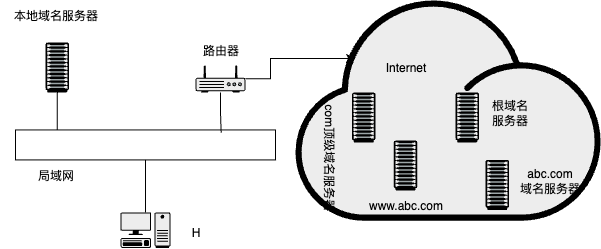
\includegraphics[scale=0.6]{计网图1.png}
    \end{figure}
    A.10ms,\ 40ms\qquad B.10ms,\ 50ms\qquad C.20ms,\ 40ms\qquad D.20ms,\ 50ms

    \item 文件传输协议(FTP)的一个主要特征是() \\
    A.允许客户指明文件的类型但不允许指明文件的格式 \\
    B.不允许客户指明文件的类型但运行指明文件的格式 \\
    C.允许客户指明文件的类型与格式 \\
    D. 不允许客户指明文件的类型与格式 

    \item 匿名FTP访问通常使用()作为用户名 \\
    A.guest\qquad B.E-mail地址\qquad C.anonymous\qquad D.主机id

    \item 下列关于POP3协议的说法,()是错误的 \\
    A.由客户端而非服务器选择接收后是否将邮件保存在服务器上
    B.登录到服务器后,发送的密码是加密的 \\
    C.协议是基于ASCII码的,不能发送二进制数据 \\
    D.一个账号在服务器上只能有一个邮件接收目录 

    \item 下面的()协议中,客户机与服务器之间采用面向无连接的协议进行通信. \\
    A.FTP\qquad B.SMTP\qquad C.DNS\qquad D.http

    \item 仅需Web服务器对HTTP报文进行响应,但不需要返回请求对象时,HTTP请求报文应该使用的方法是() \\
    A.GET\qquad B.PUT\qquad C.POST\qquad D.HEAD

    \item 下列关于Cookie的说法中,错误的是() \\
    A.Cookie存储在服务器端\qquad B.Cookie是服务器产生的\\
    C.Cookie会威胁客户的隐私\qquad D.Cookie的作用是跟踪用户的访问和状态

    \item 传输层上使用套接字的主要优点是(\qquad) 
    \begin{choices}[1]
        \task 使客户机与服务器的通信更加快捷 
        \task 能够完成点对点通信
        \task 降低服务器请求失败的可能性
        \task 当请求服务器时可以使用面向连接的协议
    \end{choices}

    \item 以下协议与其他熟知端口号的对应关系正确的是(\qquad)
    \begin{choices}
        \task DNS:80
        \task HTTP:69
        \task SMTP:20
        \task TELNET:23
    \end{choices}

    \item TCP报文中目的端口号的作用是(\qquad)
    \begin{choices}
        \task 指定服务器
        \task 指定请求的服务
        \task 指定传输方式
        \task 指定报文长度
    \end{choices}

    \item 长度为2000B的应用层数据依次封装成TCP报文段,IP数据报和以太网的帧后传送出去(不考虑前导码以及以太网帧拆分情况),
    则数据的最高传输效率为(\qquad)
    
    \item 以下说法错误的是(\qquad)
    \begin{choices}[1]
        \task UDP是无连接的,TCP是面向连接的
        \task UDP比IP多了复用分用和数据差错检测的功能
        \task 一个进程使用UDP协议,另一个进程使用TCP协议,它们可以同时使用同一端口号,
        当从网络层获取数据时,可以根据协议类型实现分用
        \task HTTP协议通信过程中,客户端使和服务端都使用80号端口
    \end{choices}

    \item 下列网络应用中,(\qquad)不适合使用UDP协议. 
    \begin{choices}[2]
        \task 客户-服务器领域
        \task 远程调用
        \task 实时多媒体应用
        \task 远程登录
    \end{choices}

    \item 以下关于UDP校验和的描述中,错误的是(\qquad)
    \begin{choices}[1]
        \task 计算校验和的时候,需要4字节对齐,若数据部分不足,需用0比特填充
        \task 校验和检查UDP的首部和数据部分
        \task 检验处UDP数据报错误的时,可以丢弃或报告上层
        \task UDP校验和能检验UDP数据报外,还能检验IP数据报的源IP地址和目的IP地址.
    \end{choices}

    \item TCP是面向字节流的传输协议,关于TCP报文段长度的表达,正确的是(\qquad)
    \begin{choices}[1]
        \task TPC报文段长度根据每次应用进程需要传输的数据块长度决定
        \task TCP报文段长度根据路径上能够传送的最大数据块长度决定
        \task TCP报文段长度根据接收方的接受能力和网络状态决定
        \task TCP报文段长度确定后,在本应用进程通信过程中保持不变
    \end{choices}

    \item 一个TCP连接的数据传输阶段,如果发送端的发送窗口由2000变成3000,意味着发送端可以发送(\qquad)
    \begin{choices}[1]
        \task 在接受到一个确认前可以发送3000个TCP报文段
        \task 在收到一个确认之前可以发送1000B
        \task 在收到一个确认之前可以发送3000B
        \task 在接受到一个确认前可以发送1000个TCP报文段
    \end{choices}

    判断正误:
    \begin{enumerate}
        \item [(1)] 网络拥塞窗口是发送端根据网络的拥塞程度和接收端的接受能力而设定的. 
        \item [(2)] 将流量控制用于TCP数据传输的原因是为了防止输入数据耗尽接收方资源
    \end{enumerate}

    \item 主机A和主机B刚建立TCP连接时候,约定最大的报文段为2KB,假设主机B的接受窗口为20KB,且保证及时
    清空缓存,拥塞门限值为16KB,RTT=10ms,在不发送拥塞的情况下.则经过(\qquad)ms主机A的发送窗口第一次为20KB.

    \item 主机甲和主机乙新建了一个TCP连接,甲的初始拥塞门限值为32KB,甲向乙始终以MSS=1KB的大小段发送数据.乙
    未该连接分配16KB接受缓存,并对每一个数据段进行确认,忽略其余延迟.若乙收到数据后全部收入缓存,不被取走,则甲从连接
    成功时刻起,未发生超时的情况下,经过4个RTT后,甲的发送窗口大小为(\qquad)
    \begin{choices}
        \task 1KB
        \task 8KB
        \task 16KB
        \task 32KB
    \end{choices}
\end{enumerate}


\section{综合题}

\newpage

\section{选择题答案}
\begin{enumerate}
    \item 选A; 套接字(socket)本质是IP地址+端口号,是传输层的T-SAP(传输服务访问点). 传输层并不提供{\color{red}点到点,而是提供端到端(进程到进程)间的通信}
    需要注意并非TCP专用套接字,UDP也使用. 
    \item 选D; 应用层协议端口号与对应传输层协议需要多记
    \item 选B; 服务器由IP地址决定,传输方式由所使用的协议决定,报文长度由报文首部决定
    \item 97.19\%; 需要熟练记忆各协议首部的长度以及关键参数 
    \item D; HTTP协议的客户端端口为动态分配,服务器为熟知端口80
    \item D; UDP的特点是效率高,开销小,延迟低;但不保证数据准确.通常不用于需要持久性连接的应用.
    \item A; 计算校验和需要{\color{red} 2字节对齐而非4字节对齐} 
    \item C;
    \item C; 这题并不严谨,主要是记录TCP是以字节为单位控制窗口而非TCP端 \\
    判断正误: 错, 网络拥塞窗口->发送窗口 \\
    判断正误: 对
    \item 50ms; 注意MSS=2KB, 其变化规律应该是4KB->8KB->16KB(到达上限)->18KB-20KB 注意后面每次是加1MSS而非1KB
    \item A; 题设很长注意抓关键点{\color{red} 收入数据后不被取走},发送窗口由接收方窗口大小和拥塞窗口大小的较小值决定.
\end{enumerate}
\ifx\allfiles\undefined
\end{document}
\fi